\documentclass[11pt,a4paper]{article}
\PassOptionsToPackage{obeyspaces,spaces}{url}
\usepackage[margin=22mm]{geometry}
\usepackage[T1]{fontenc}
\usepackage{lmodern,tabularx,booktabs,xcolor}
\usepackage{graphicx,listings,xltabular,enumitem,caption,needspace,float}
\usepackage[hidelinks]{hyperref}
\setlength{\parindent}{0pt}\setlength{\parskip}{6pt}
% Template field macro (the grey placeholder styling is removed).
\newcommand{\entry}[1]{\par\textbf{#1:} }
\newcommand{\code}[1]{\nolinkurl{#1}}
\makeatletter
\g@addto@macro{\UrlBreaks}{\do\_\do\-\do\.}
\makeatother
\renewcommand{\arraystretch}{1.15}
\setlength{\emergencystretch}{2.5em}
\setlist{nosep,leftmargin=1.4em}
\captionsetup{font=small,labelfont=bf}
\lstset{basicstyle=\ttfamily\footnotesize,columns=fullflexible,keepspaces=true,
  frame=single,framerule=0.3pt,rulecolor=\color{gray},numbers=left,numberstyle=\tiny\color{gray},
  numbersep=6pt,xleftmargin=1.5em,breaklines=true,showstringspaces=false,upquote=true}
\begin{document}
\begin{center}\Large\textbf{23CSE455 Design Patterns}\\[4pt]\LARGE Case Study Report\end{center}

\entry{Team}A1
\entry{Case study}Food delivery application built with Django: discovery, evolution and cross-language comparison of the design patterns in a working campus food-ordering system.
\entry{Application}\href{https://github.com/HarshavardhanVemali/campus-food-ordering}{HarshavardhanVemali/campus-food-ordering} (``Canteen Management System'', MIT licence). Approved by the course faculty as Team A1's application.
\entry{Date}2026-10-11
\par\textbf{Submission repository:} \href{https://github.com/aswathymohan-amrita/23CSE455_DP_CaseStudy}{23CSE455\_DP\_CaseStudy}, folder \code{A1/}\par
\textbf{Students}\par
\begin{tabularx}{\linewidth}{@{}llX@{}}\toprule
Roll number & Student name & Batch\\\midrule
AM.SC.U4CSE23001 & Aadil Nizar & CSE A\\
AM.SC.U4CSE23007 & Adil Najeem & CSE A\\
AM.SC.U4CSE23014 & Athul Yesudas & CSE A\\
AM.SC.U4CSE23039 & Hima C & CSE A\\
AM.SC.U4CSE23046 & M Krishnapriya & CSE A\\
AM.SC.U4CSE23053 & Muhammed Faais A & CSE A\\\bottomrule
\end{tabularx}

\section{Application and architecture}
\entry{Original source}Repository \url{https://github.com/HarshavardhanVemali/campus-food-ordering} (\code{main}). There is no release tag, so the snapshot is identified by commit \code{83998629e633}\allowbreak\code{594037cfa25e}\allowbreak\code{583542f9f6f0f968}. The commit archive (SHA-256 \code{104b48ea...0263c}, \code{data/provenance/provenance.json}) contains 170 files, and each file's hash is listed in \code{data/provenance/baseline-files.sha256.json}. The copy in \code{data/code/baseline_83998629/} keeps 167 files byte-identical. Two files carry one-line credential redactions (\code{data/provenance/REDACTIONS.md}), and a 15~MB stock video is left out of the package; \code{data/code/verify_baseline.py} checks all three groups. The team's earlier download (\code{campus-food-ordering-main.zip}) has the same content, and a repository screenshot from 2026-09-12 (\code{data/provenance/github_repository_page_2026-09-12.png}) shows the same short hash, \code{8399862}. The repository page was captured on 2026-09-12 and the commit archive was fetched on 2026-10-11. Licence: MIT (\code{LICENSE}, copyright 2025 Harshavardhan Vemali).

\entry{Environment}Python with Django and Django Channels (ASGI through Daphne); SQLite (\code{settings.DATABASES}); the Channels \code{InMemoryChannelLayer} (\code{canteen/settings.py:131-135}); django-allauth and social-auth for Google sign-in; Firebase Admin for push messages; and the PhonePe and PayU payment SDKs. \code{requirements.txt} pins 99 packages, among them Django 6.0.4, channels 4.3.2, daphne 4.2.1, django-allauth 65.16.1, firebase-admin 7.4.0 and phonepe-sdk 1.1.0. The upstream README mentions Django 5.1 and Redis, but the pinned requirements and \code{settings.py} do not use them, and this report follows the code. CH01 was validated with Python 3.12.14, Django 6.0.4, Channels 4.3.2 and SQLite 3.53.1 (\code{Part2/changes/Change1/evidence/runtime-versions.txt}; full package list in \code{environment-freeze.txt}). Part~3 used OpenJDK 21.0.12.1, CPython 3.13.16, Node.js 22.22.0 and g++ 13.3.0 (\code{Part3/evidence/toolchain_versions.txt}).

\entry{Scope}The application consists of one Django app, \code{canteenapp}, and the project package \code{canteen}. Inspected in detail: \code{canteenapp/models.py} (629 lines), \code{views.py} (5{,}363 lines), \code{consumers.py} (946 lines), \code{signals.py}, \code{apps.py}, \code{routing.py}, \code{canteen/settings.py}, \code{urls.py}, \code{asgi.py} and the template \code{adminassignorder.html}. A reproducible scan (\code{Part1/evidence/scan_candidates.sh}) covered every Python module of \code{canteenapp}. Participants were verified in three areas that the case study and its changes depend on: item availability, the order-status lifecycle and delivery assignment. Excluded: the other 62 templates and the static CSS and JavaScript, which hold presentation only; the 17 migration files, which are generated schema history; and the internals of Django, Channels and social-auth, whose roles are taken from their documentation \cite{djsignals,channels}. The payment and notification code was read only as far as needed to judge the Facade, Adapter and Singleton candidates.

\entry{Architecture}Figure~\ref{fig:arch} shows the components. \code{canteen/asgi.py} sends plain HTTP to Django and passes WebSocket connections through \code{AuthMiddlewareStack} to the consumers listed in \code{canteenapp/routing.py}. Most business logic lives in function-based views, although models such as \code{Order} also calculate prices and handle stock. An order-status update shows how the parts work together:
\begin{enumerate}
\item an administrator's page posts JSON to \code{/adminupdateorderstatus/};
\item the view checks that the status does not move backwards (\code{get_status_index}) and saves the \code{Order};
\item it calls \code{group_send} on the channel layer for the admin, restaurant and delivery groups;
\item Channels delivers each event to every consumer in the group and calls the handler named by the event type;
\item each handler re-reads the relevant orders and pushes JSON over the WebSocket to its browser.
\end{enumerate}
A second, synchronous path runs inside the ORM: saving an \code{Item} emits \code{post_save}, and a receiver deletes cart rows for unavailable items.

\begin{figure}[!htbp]\centering
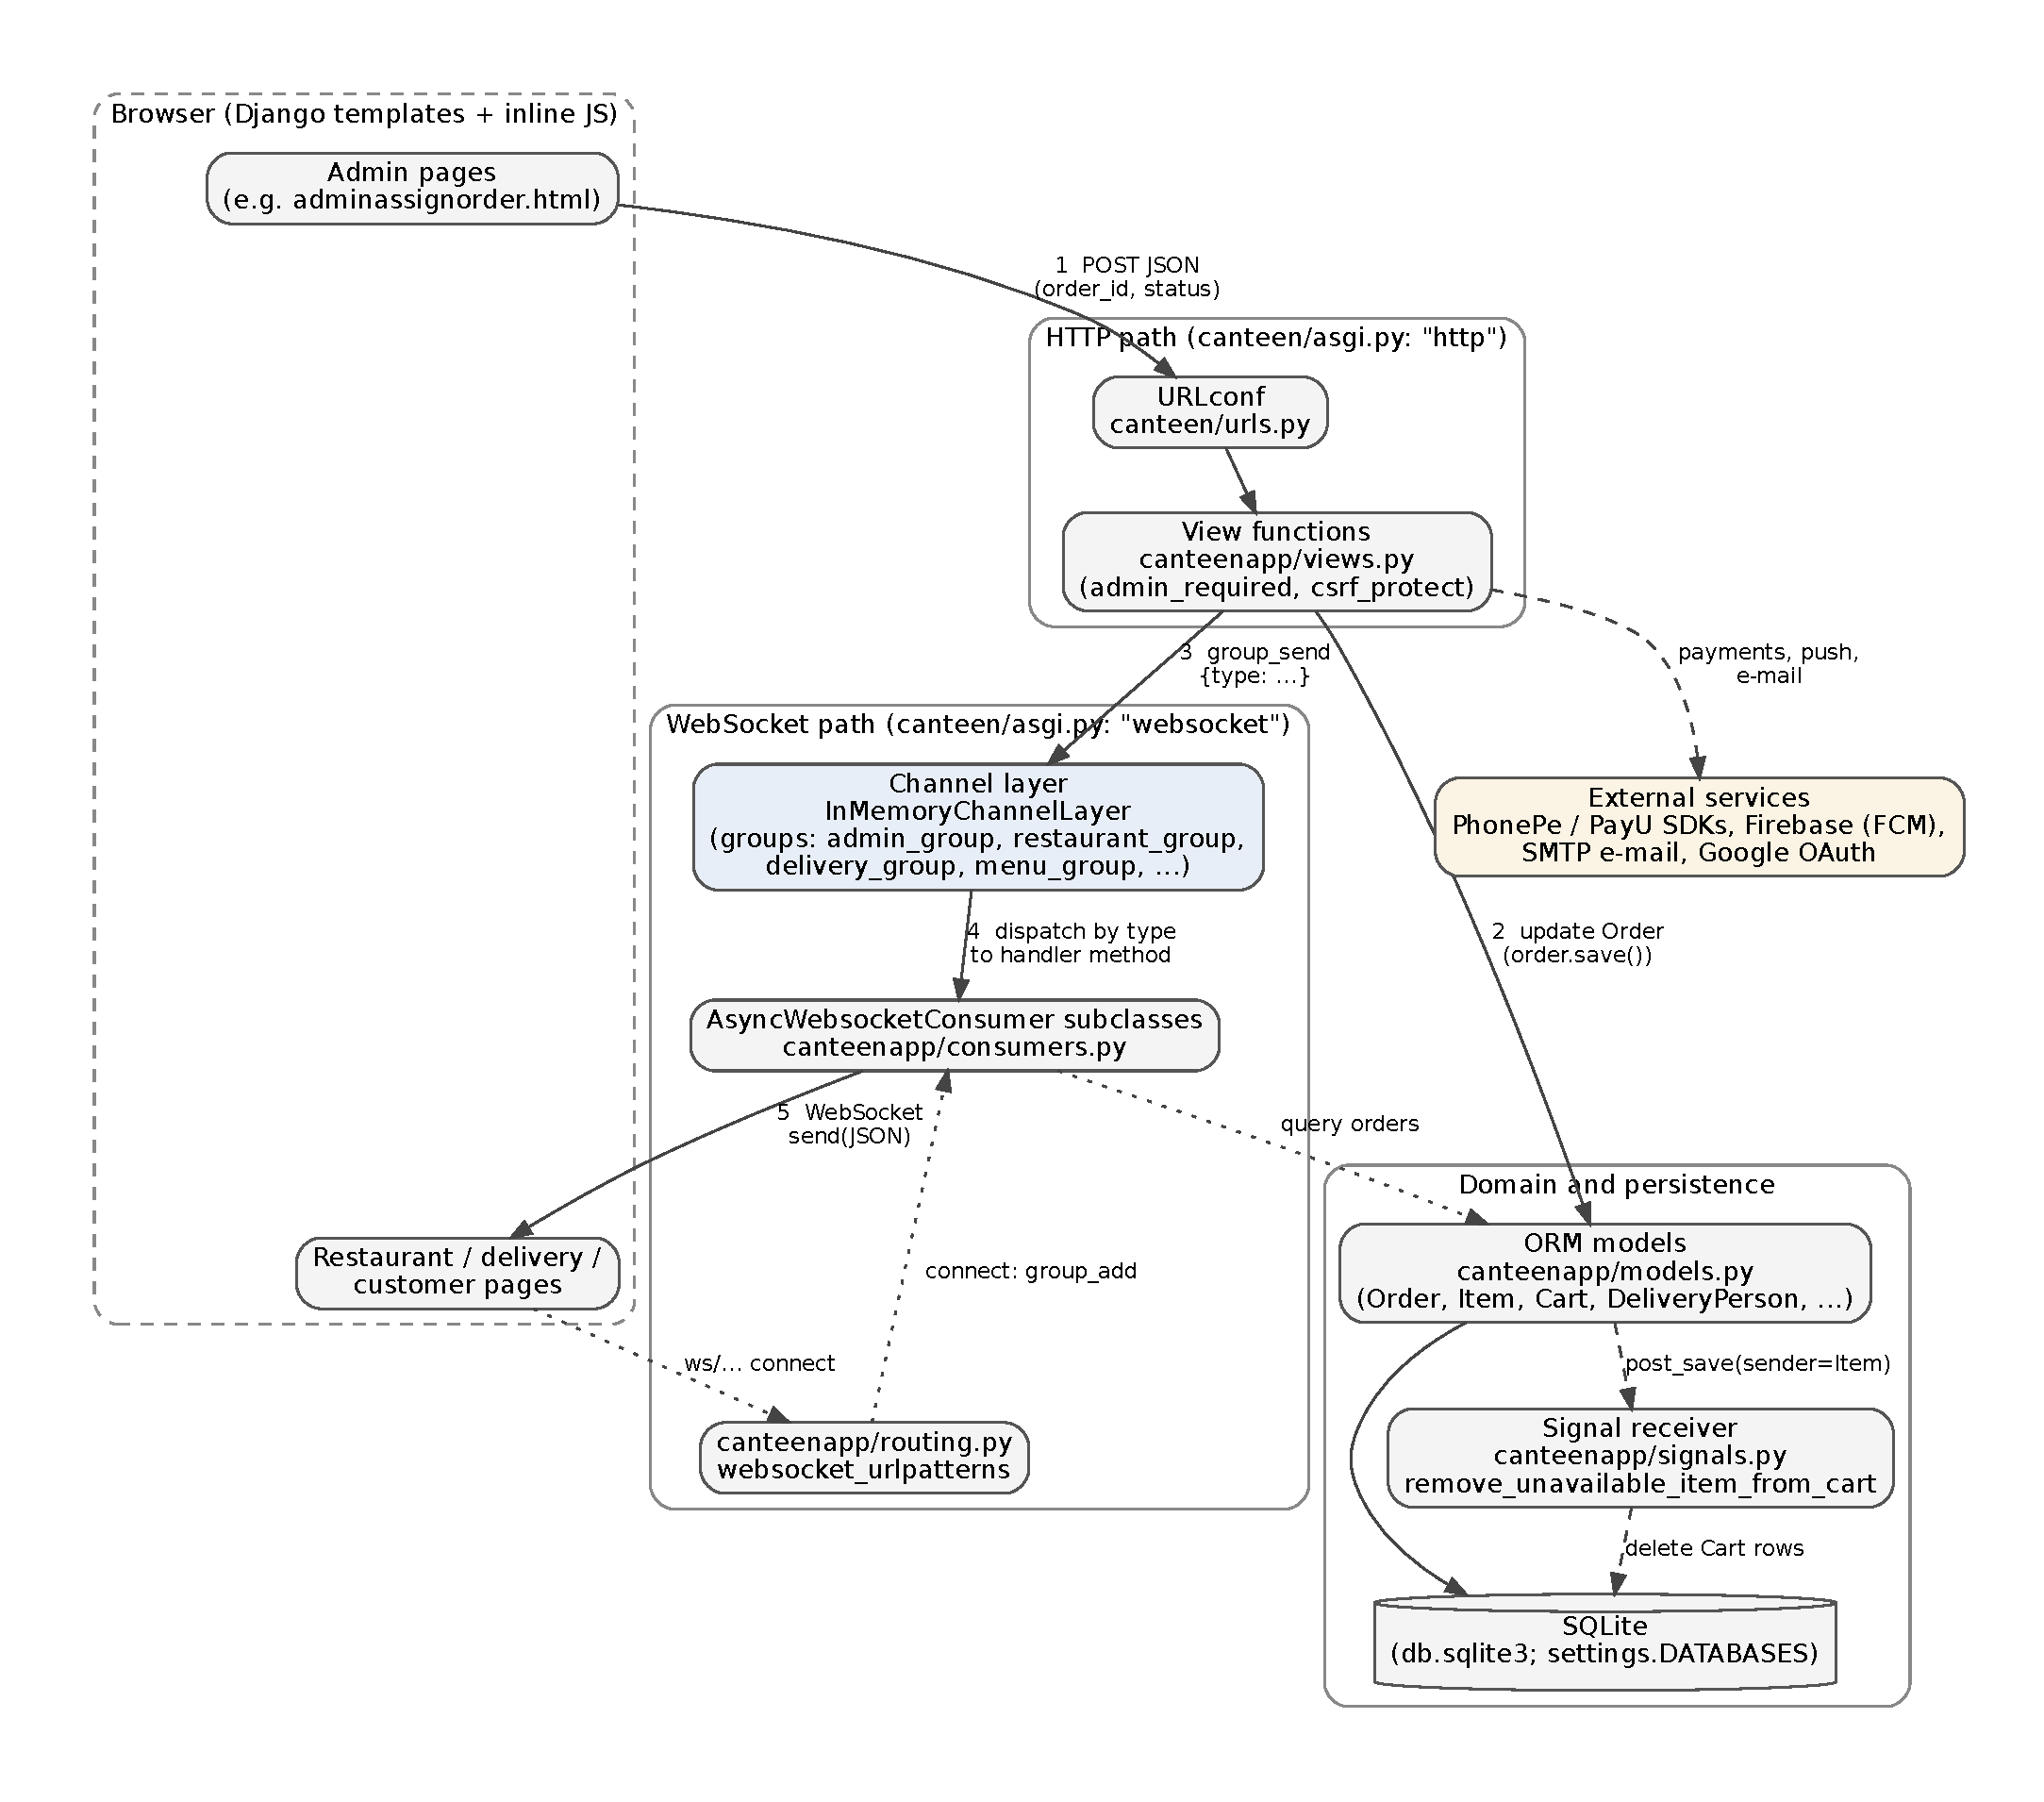
\includegraphics[width=\linewidth]{Part1/pattern_architecture/architecture.pdf}
\caption{Components and the order-status request/event flow at commit 83998629. Source: \code{Part1/pattern_architecture/architecture.dot} (Graphviz), with the rendered PDF and PNG beside it.}\label{fig:arch}
\end{figure}

\entry{Run instructions}The upstream setup steps are in \code{data/code/baseline_83998629/README.md}: create a virtual environment, run \code{pip install -r requirements.txt}, create \code{.env} from \code{.env.example}, apply migrations and start the ASGI server. Followed literally, the installation fails: \code{phonepe-sdk} is not on the default package index, \code{psycopg2} needs \code{pg_config}, and several pinned packages conflict (\code{Part2/changes/Change1/evidence/install*.log}). A validation environment was therefore assembled as recorded in \code{Part2/changes/Change1/verification/commands.md}. In that environment \code{python manage.py check} exits 0 with one deprecation warning (\code{ACCOUNT_EMAIL_REQUIRED}) and a message that the Firebase service-account file is missing, and \code{python manage.py makemigrations --check --dry-run} reports no changes. The development server was not started for this study.

\section{Part 1 Pattern discovery}
\entry{Method}Candidates came from three sources: the team's earlier analysis note (\code{Part1/llm/historical_note_pattern_analysis.md}), a reading of the modules in scope, and a scripted scan of the baseline (\code{Part1/evidence/candidate_scan.txt}). The scan looked for signal receivers, Channels subscriptions and publications, routed consumers, abstract classes, class names suggesting GoF roles, status tables, module-level singletons, the social-auth pipeline and access-control decorators. A candidate was confirmed only when three conditions held:
\begin{enumerate}
\item every role of the pattern mapped to application code or to a documented framework mechanism;
\item the calls forming the collaboration could be traced in both directions;
\item at least one concrete participant varied independently of the code that triggers it.
\end{enumerate}
A class name, an inheritance link or an LLM statement was not accepted on its own. Line ranges come from Python's \code{ast} module and include decorators.

\subsection{Totals at the baseline}
\entry{Confirmed pattern types}1: Observer.
\entry{Confirmed pattern instances}2: Item Unavailability Cart Cleanup and Order Status Broadcast.
\entry{Concrete participant classes}3: \code{AdminOrderConsumer}, \code{RestaurantOrderConsumer} and \code{DeliveryOrderConsumer}. The concrete observer of the first instance is a module-level function, so it adds no class.
\entry{Unique participant symbols}13. One symbol is counted for each class, module-level function or module-level object mapped to a GoF role. Methods count with their class, and a symbol shared between instances counts once. Supporting rows in the mapping tables (registration, routing, callers, affected data) are not counted. The first instance contributes 3 symbols and the second 10. Three of the 13 are framework symbols: \code{post_save}, \code{InMemoryChannelLayer} and \code{AsyncWebsocketConsumer}.
\entry{Rejected and uncertain candidates}12 rejected and 2 uncertain (Table~\ref{tab:rejected}). Observation scope: all Python modules of \code{canteenapp} at commit 83998629, scanned on 2026-10-11, with participant-level checks in the three areas named under Scope.

\subsection{Pattern inventory}
\begin{tabularx}{\linewidth}{@{}lXll@{}}\toprule
Pattern type & Instance names & Instances & Concrete classes\\\midrule
Observer & Item Unavailability Cart Cleanup; Order Status Broadcast & 2 & 3\\\bottomrule
\end{tabularx}

Canonical records: \code{data/patterns.csv} and \code{data/pattern_counts.csv}. The Strategy collaboration found in the evolved code is introduced by CH01 and is counted only in that snapshot (Section~\ref{sec:counts}).

\subsection{One record for each pattern instance}
\entry{Instance name}Item Unavailability Cart Cleanup
\entry{Pattern type and category}Observer; GoF behavioural pattern \cite{gof}, implemented through Django's signal dispatcher (framework idiom).
\entry{Purpose and origin}When an item's stock reaches zero, the item must disappear from every customer's cart. The code that changes stock (checkout and four item-editing views) should not need to know that carts exist. The application supplies the subject and the observer, and Django supplies the dispatch mechanism.

\needspace{12\baselineskip}\textbf{Participant mapping}\par\nopagebreak
\begin{tabularx}{\linewidth}{@{}p{0.19\linewidth}XX@{}}\toprule
Pattern role & Actual class, interface and function & File and line range\\\midrule
Subject & \code{django.db.models.signals.post_save}, a \code{django.dispatch.Signal}: attach with \code{@receiver}/\code{connect()}, notify with \code{send()} & Django 6.0.4 (framework)\\
ConcreteSubject & \code{canteenapp.models.Item}; \code{Item.save()} derives \code{is_available} and calls \code{Model.save()}, which sends \code{post_save} & \code{data/code/baseline_83998629/canteenapp/models.py:123-149} (save 144--149)\\
Observer & not separately declared; Django's receiver protocol \code{(sender, instance, **kwargs)} & ---\\
ConcreteObserver & \code{canteenapp.signals.remove_unavailable_item_from_cart} (function) & \code{.../canteenapp/signals.py:52-57}\\
Registration (supporting) & \code{CanteenappConfig.ready()} imports \code{canteenapp.signals} & \code{.../canteenapp/apps.py:3-8}\\
Affected data (supporting) & \code{canteenapp.models.Cart} & \code{.../canteenapp/models.py:151-168}\\
Callers (supporting) & \code{Order.create_order_from_cart}; \code{adminupdateitem}, \code{adminupdateitemimage}, \code{restaurantupdateitem}, \code{restaurantupdateitemimage} & \code{models.py:340, 355, 358}; \code{views.py:996, 1053, 3960, 4015}\\\bottomrule
\end{tabularx}

\entry{Evidence}The subject sets its own availability before saving (\code{models.py}):
\begin{lstlisting}[language=Python,firstnumber=144]
    def save(self,*args,**kwargs):
        if self.count==0:
            self.is_available=False
        else:
           self.is_available = True
        super().save(*args,**kwargs)
\end{lstlisting}
The observer subscribes to that sender only and acts only on the unavailable state (\code{signals.py}):
\begin{lstlisting}[language=Python,firstnumber=52]
@receiver(post_save, sender='canteenapp.Item')
def remove_unavailable_item_from_cart(sender, instance, **kwargs):
    from .models import Cart

    if not instance.is_available:
        Cart.objects.filter(item=instance).delete()
\end{lstlisting}
\code{CanteenappConfig.ready()} imports the signals module, which is how Django recommends connecting decorated receivers \cite{djsignals}. None of the five callers mentions \code{Cart}; each one only calls \code{item.save()}. Checkout contains one subtle point. Line~339 assigns an \code{F('count') - quantity} expression, so the comparison in \code{Item.save()} triggered at line~340 is not a numeric test. The method then re-reads the item and saves it again (lines 352--358), and that second save is the one that announces unavailability correctly.
\entry{Diagram}Figure~\ref{fig:obs1}; source \code{Part1/pattern_architecture/observer_item_cart_cleanup.dot}, with the rendered PDF and PNG beside it.
\entry{Verification}Confirmed. Every role maps either to code or to Django's documented signal API. The notification path runs from \code{Item.save()} through \code{post_save} to the receiver, and the subject holds no reference to its observer. The repository has no test for this path (\code{canteenapp/tests.py} is a placeholder), so the classification rests on the source. Two alternatives were considered. A direct call in each view would repeat the cleanup in five places, and a model method would couple \code{Item} to \code{Cart}. The mechanism has one consequence that matters for later changes: \code{QuerySet.update()} does not send \code{post_save}, so a bulk stock update would bypass the cleanup. The baseline contains no such update.

\begin{figure}[!htbp]\centering
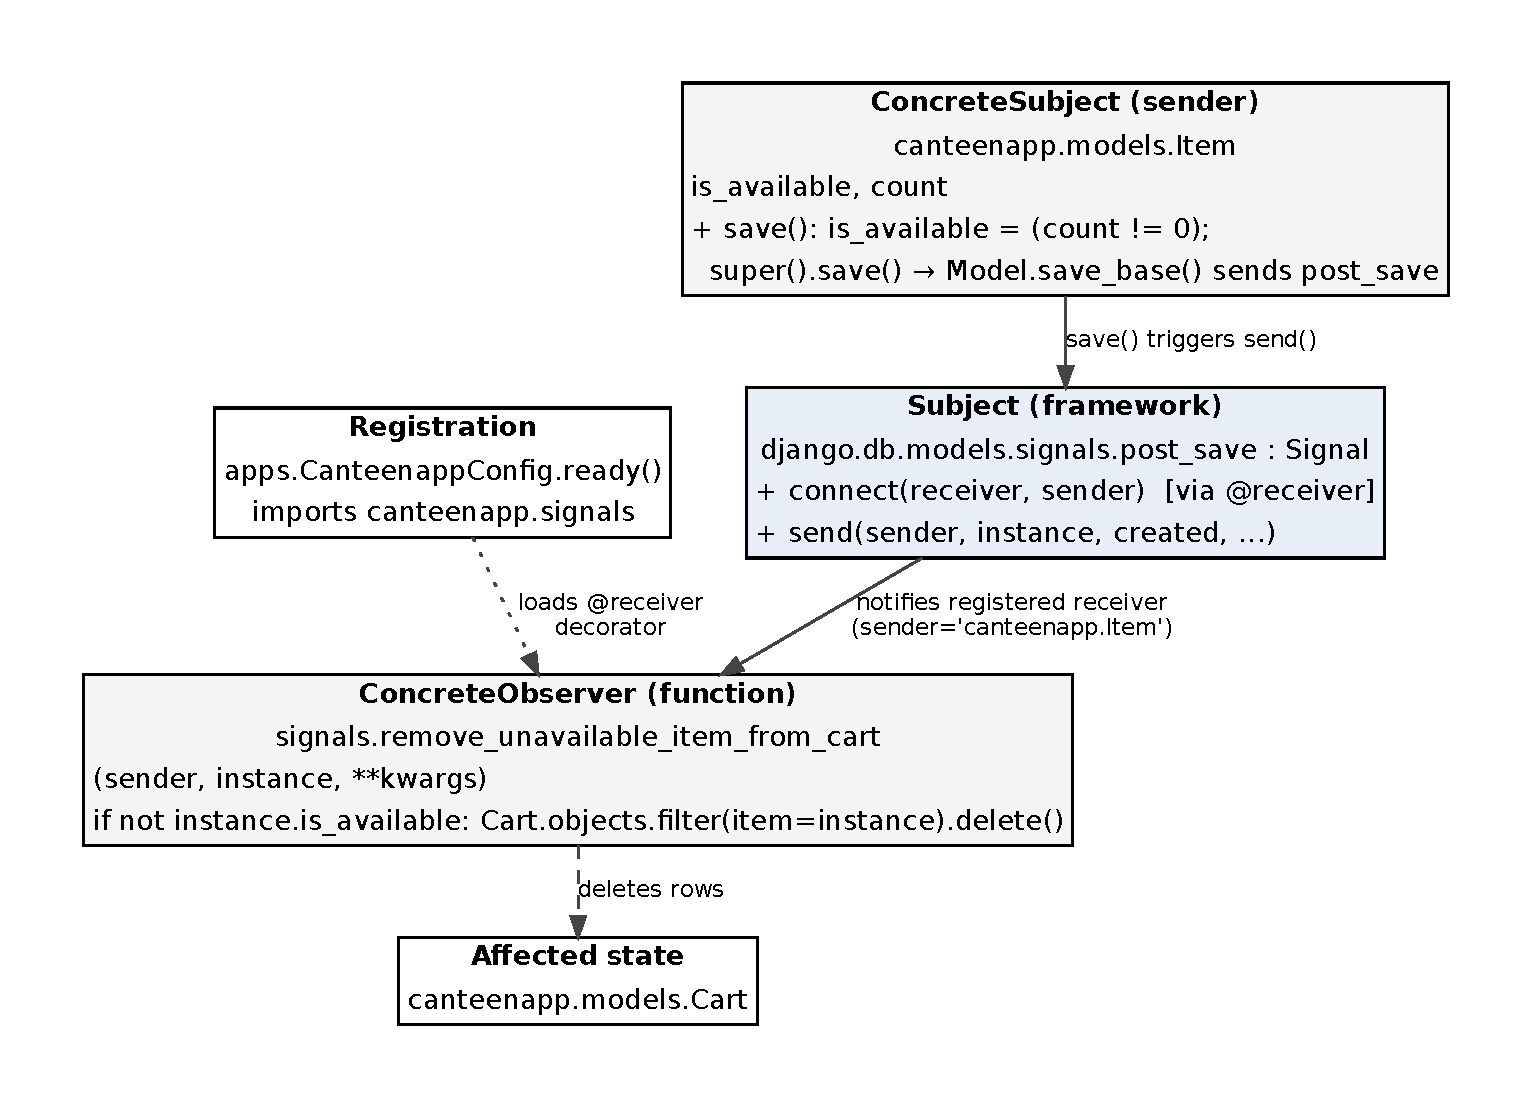
\includegraphics[width=0.7\linewidth]{Part1/pattern_architecture/observer_item_cart_cleanup.pdf}
\caption{Item Unavailability Cart Cleanup: roles mapped to Django and application symbols.}\label{fig:obs1}
\end{figure}

\entry{Instance name}Order Status Broadcast
\entry{Pattern type and category}Observer in its publish--subscribe form; GoF behavioural pattern, mediated by Django Channels groups (framework-provided registry).
\entry{Purpose and origin}A status change must refresh several live dashboards (administrator, restaurant and delivery staff) without the view knowing which browsers are connected. The application supplies the notifiers and the concrete observers, and Channels handles registration and delivery.

\needspace{12\baselineskip}\textbf{Participant mapping}\par\nopagebreak
\begin{tabularx}{\linewidth}{@{}p{0.19\linewidth}XX@{}}\toprule
Pattern role & Actual class, interface and function & File and line range\\\midrule
Subject (registry) & not declared by the application; \code{channels.layers.InMemoryChannelLayer} keeps group membership (\code{group_add}, \code{group_discard}, \code{group_send}) & \code{canteen/settings.py:131-135}; channels 4.3.2\\
ConcreteSubject (notifiers) & view functions rather than a class: \code{adminupdateorderstatus} (representative), \code{deliveryupdatedeliverystatus}, \code{restaurantupdateorderstatus}, \code{restaurantplaceorder}, \code{phonepe_callback} & \code{views.py:2124-2251}, \code{3317-3432}, \code{4356-4483}, \code{4552-4654}, \code{4797-4974}\\
Observer & \code{channels.generic.websocket.AsyncWebsocketConsumer}; an event's \code{type} selects the handler method of the same name & channels 4.3.2\\
ConcreteObserver & \code{AdminOrderConsumer} (group \code{admin_group}) & \code{consumers.py:350-460}\\
ConcreteObserver & \code{RestaurantOrderConsumer} (\code{restaurant_group}) & \code{consumers.py:462-587}\\
ConcreteObserver & \code{DeliveryOrderConsumer} (\code{delivery_group}) & \code{consumers.py:589-688}\\
Wiring (supporting) & \code{websocket_urlpatterns}; \code{canteen.asgi.application} & \code{routing.py:10-12}; \code{asgi.py:20-29}\\\bottomrule
\end{tabularx}

\entry{Evidence}Each consumer attaches itself when the socket connects and detaches when it closes (\code{consumers.py}):
\begin{lstlisting}[language=Python,firstnumber=351]
    async def connect(self):
        user = self.scope.get('user')
        if user and user.is_authenticated and user.role == 'admin':
            self.group_name = 'admin_group'
            await self.channel_layer.group_add(self.group_name, self.channel_name)
            await self.accept()
        else:
            await self.close()
\end{lstlisting}
The notifier changes the order's state and then publishes events that carry only a type (\code{views.py}):
\begin{lstlisting}[language=Python,firstnumber=2168]
            order.status = status
            order.save()
            async_to_sync(channel_layer.group_send)(
                    'admin_group',
                    {
                        "type": 'admin_all_order'
                    }
             )
\end{lstlisting}
\code{adminupdateorderstatus} sends eight such events to the three groups (lines 2170--2218). Channels calls the consumer method whose name equals the event type \cite{channels}. For example, \code{AdminOrderConsumer.admin_all_order} (lines 365--371) re-queries the orders and sends them to the browser. The events carry no data and each observer fetches what it needs, which is the pull model described by GoF.
\entry{Diagram}Figure~\ref{fig:obs2}; source \code{Part1/pattern_architecture/observer_order_status_broadcast.dot}.
\entry{Verification}Confirmed as Observer, with one qualification. GoF lists Publish--Subscribe as another name for Observer and describes a ChangeManager that keeps the subject--observer mapping on the subject's behalf \cite{gof}; here the channel layer's groups play that part. The collaboration is not the strict form, in which a subject object stores and calls its observers. No application class holds the list, the subject role is spread over five view functions, events are dictionaries, delivery is asynchronous, and the in-memory layer works only within one process \cite{channels}. Under a strict reading it would be a framework-mediated Publish--Subscribe Channel \cite{eip}, with the same participants and counts. Reading the code shows one inefficiency: every status change sends all eight events regardless of the transition, so each connected administrator runs three order queries per update.

\begin{figure}[!htbp]\centering
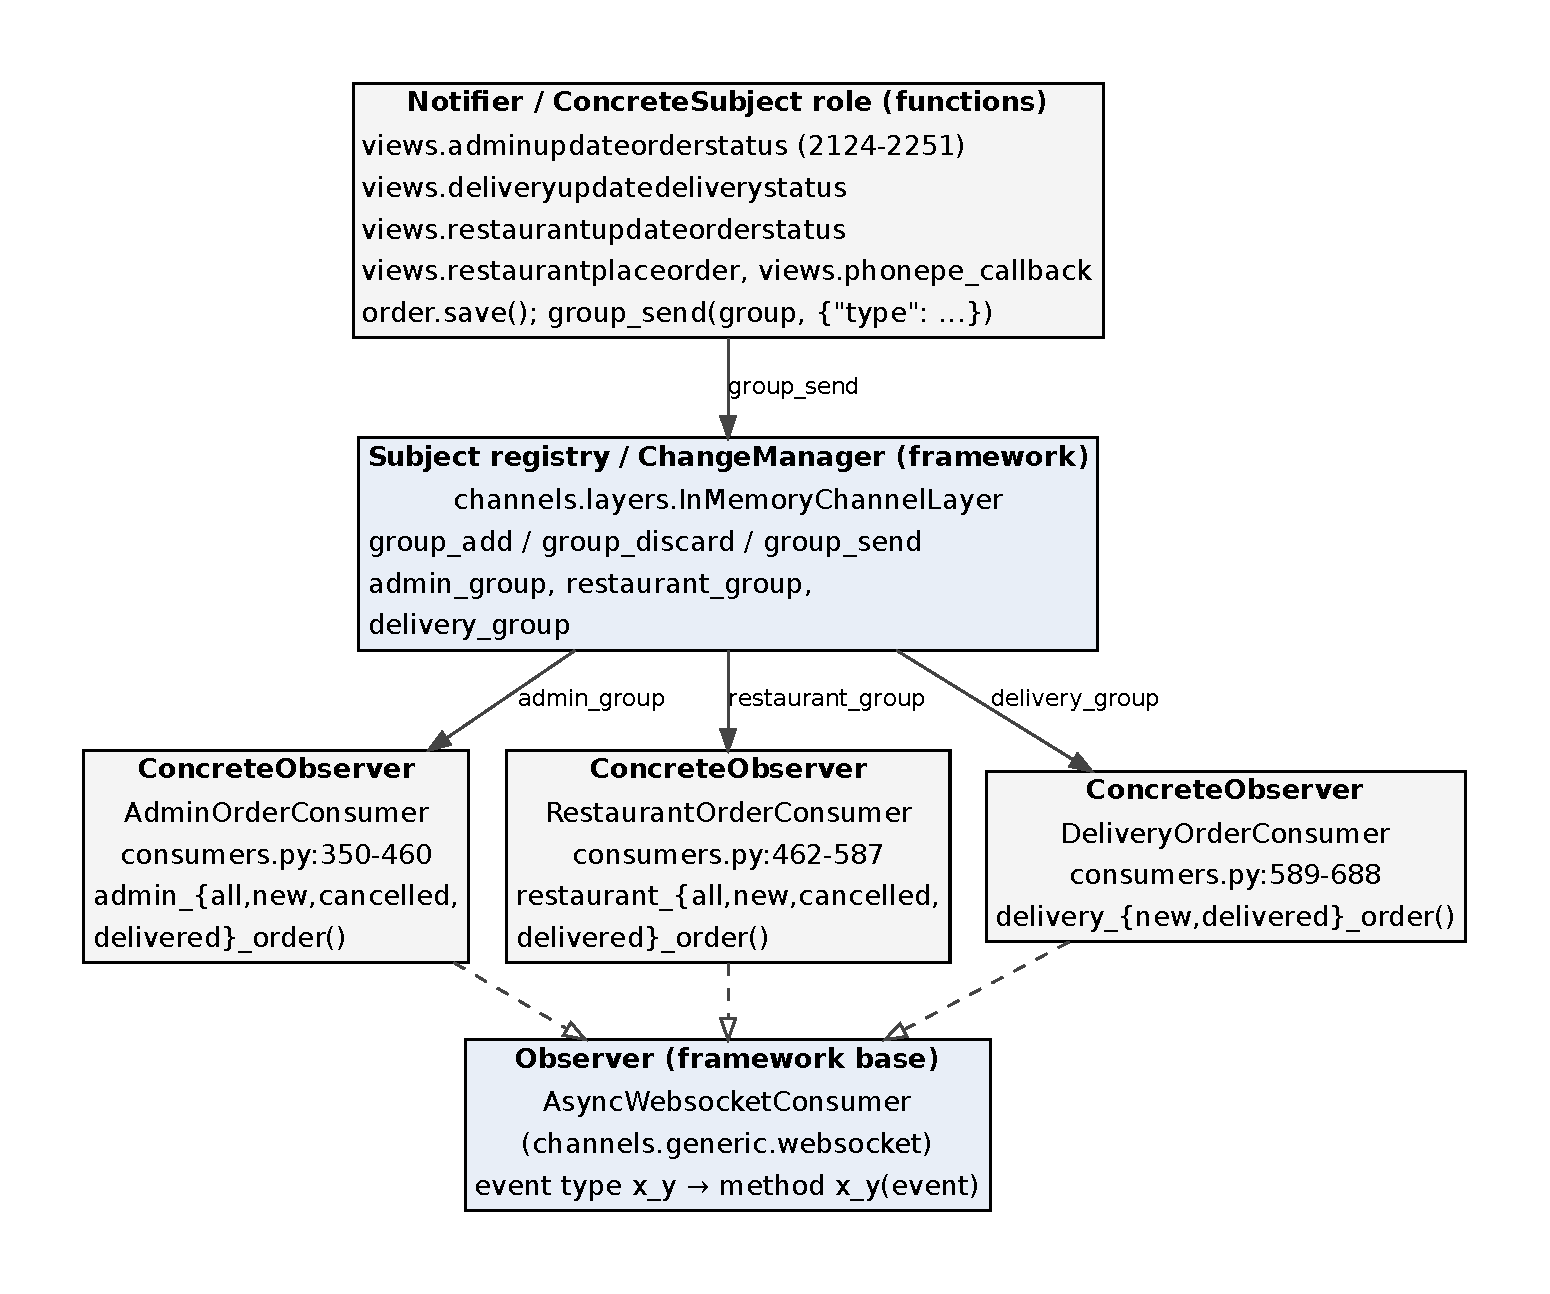
\includegraphics[width=0.7\linewidth]{Part1/pattern_architecture/observer_order_status_broadcast.pdf}
\caption{Order Status Broadcast: notifiers, framework registry and concrete observers.}\label{fig:obs2}
\end{figure}

\begin{xltabular}{\linewidth}{@{}p{0.31\linewidth}lX@{}}
\caption{Rejected and uncertain candidates at the baseline (evidence: \code{Part1/evidence/candidate_scan.txt}).}\label{tab:rejected}\\\toprule
Candidate & Status & Reason\\\midrule\endfirsthead
\toprule Candidate & Status & Reason\\\midrule\endhead
Strategy: manual delivery assignment (\code{views.py:1788-1821}) & rejected & One hard-coded lookup by the e-mail sent from the page; there is no family of algorithms and no interchangeable object.\\
Strategy: delivery-type branching (\code{Order.get_status_display}, \code{Order.add_additional_charges}, \code{get_status_index}) & rejected & \code{if}/\code{elif} on \code{delivery_type}; no strategy objects.\\
State: order status workflow (\code{models.py:260-284}, \code{views.py:2112-2122, 2161-2165}) & rejected & The state is a string checked against choice lists and an index; no state class carries behaviour.\\
Singleton: \code{phonepe_client} (\code{views.py:4701}) & rejected & A module-level object; nothing controls instantiation.\\
Facade: payment and checkout views & rejected & Long view functions coordinate several subsystems, but no class offers a simplified interface to them.\\
Adapter: PhonePe and PayU integration & rejected & Each SDK is called directly from views; there is no common gateway interface.\\
Factory: order and payment creation & rejected & Ordinary constructor and ORM \code{create()} calls.\\
Command: view functions & rejected & No request objects, invoker or undo.\\
Repository: data access & rejected & The ORM is used directly; there is no repository abstraction.\\
Template Method: \code{save()} overrides, consumer hooks & rejected & Hooks of framework base classes; the skeleton belongs to Django or Channels, not to the application.\\
Decorator: \code{admin_required}, \code{user_required} (\code{views.py:81-97}) & rejected & Function wrappers around \code{user_passes_test}; no component interface or decorator objects.\\
Observer: delivery assignment notification (\code{views.py:1811-1818}, group \code{delivery_person_<id>}) & rejected & Its only subscriber, \code{CustomerOrderConsumer}, sits inside a string literal (\code{consumers.py:691-848}) and is not routed, so no live observer exists.\\
Observer (publish--subscribe): menu, item, cart, price, search and notification groups & uncertain & Same mechanism as Order Status Broadcast across eight further groups (87 \code{group_send} calls in 23 view functions overall); their participants were not mapped group by group within this scope.\\
Pipeline / Chain of Responsibility: \code{SOCIAL_AUTH_PIPELINE} step \code{create_unique_username} (\code{settings.py:65-75}, \code{signals.py:7-50}) & uncertain & social-auth defines the pipeline and the application adds one step; whether a step can end the chain was not checked in the library source.\\\bottomrule
\end{xltabular}

\section{Part 2 Evolution and refactoring}\label{sec:part2}
\entry{Change and acceptance criteria}\textbf{CH01, interchangeable delivery-assignment policies.} An administrator assigning a confirmed delivery order should be able to choose how the delivery person is picked, and a new rule should not require rewriting the assignment view. Acceptance criteria, each covered by tests in the CH01 package:
\begin{enumerate}
\item the existing manual payload \texttt{\{"order\_id", "delivery\_personnel"\}} still assigns the chosen person, sets the status to \code{shipped} and returns \code{success: true};
\item the payload \texttt{\{"order\_id", "policy": "least\_workload"\}} assigns, without an e-mail, the eligible person with the fewest unfinished delivery orders, breaking ties by the lowest user ID;
\item only active, non-superuser accounts with the role \code{delivery_person} and the \code{canteenapp.is_deliveryperson} permission, held directly or through a group, are eligible;
\item only orders still in the assignment queue (delivery type, confirmed, confirmed by the customer, unassigned) can be assigned;
\item malformed input returns 400, a missing order 404, a stale order or an empty candidate set 409, and a database failure 503;
\item the admin page offers both policies with manual as the default, the existing channel event is still sent, and no schema change is needed.
\end{enumerate}
\entry{Before and after}Before: commit \code{83998629}. After: the working tree \code{data/code/evolved_CH01/} and the unified diff \code{Part2/changes/Change1/CH01.diff}; CH01 was not committed to Git. Applying the diff to a fresh copy of the baseline reproduces the four changed files byte for byte (\code{Part2/changes/Change1/rerun_2026-10-11/RECHECKS.md}). Changed paths:
\begin{itemize}
\item \code{canteenapp/delivery_assignment.py} (added);
\item \code{canteenapp/views.py} (modified);
\item \code{canteenapp/templates/adminassignorder.html} (modified);
\item \code{canteenapp/test_delivery_assignment.py} (added).
\end{itemize}
Models, migrations, settings, consumers, signals, routes and \code{requirements.txt} are unchanged (\code{data/provenance/changed-files.json}).

\entry{Implementation and tests}The new module declares the policy abstraction:
\begin{lstlisting}[language=Python,firstnumber=36]
class DeliveryAssignmentPolicy(ABC):
    @abstractmethod
    def select(self, candidates, *, email=None):
        """Return one eligible DeliveryPerson, or raise AssignmentError."""
\end{lstlisting}
\code{ManualAssignmentPolicy} (lines 42--49) returns the eligible candidate with the supplied e-mail. \code{LeastWorkloadAssignmentPolicy} (lines 52--66) annotates each candidate with a distinct count of assigned delivery orders that are neither \code{delivered} nor \code{cancelled}, then orders by that count and by primary key. An unknown status value therefore counts as unfinished work, which is the cautious choice. \code{DeliveryAssignmentService} is the context. Inside one transaction it checks that the order is still assignable, delegates the choice and writes through a conditional update that repeats the eligibility filter:
\begin{lstlisting}[language=Python,firstnumber=101]
        if not assignable.exists():
            raise AssignmentError("Order is no longer eligible for assignment.", 409)
        person = self.policy.select(eligible_delivery_people(), email=email)
        updated_at = timezone.now()
        # Guard the write as well: SQLite does not implement SELECT FOR UPDATE.
        if assignable.update(delivery_person=person, status="shipped", updated_at=updated_at) != 1:
            raise AssignmentError("Order changed; reload before assigning again.", 409)
\end{lstlisting}
The view now:
\begin{itemize}
\item validates the JSON body;
\item looks up the policy by name with \code{get_assignment_policy(policy_name)}, defaulting to \code{manual} (\code{views.py:1815});
\item maps each \code{AssignmentError} to its HTTP status;
\item schedules the existing \code{delivery_person_<id>}/\code{new_order} event with \code{transaction.on_commit(..., robust=True)}, so a notification failure is logged rather than reported as a failed assignment.
\end{itemize}
The page gained a policy selector and disables the manual drop-down in automatic mode. It now submits the order selected in \code{ordersData[currentOrderIndex]} instead of reading a duplicated \code{orderid} element, ignores repeated clicks and shows server messages. A CSRF test exposed a missing cookie on the assignment page, so \code{adminassignorder} now sets it.

Commands and results (working directory \code{CH01/working}; logs in \code{Part2/changes/Change1/evidence/}):

\begin{tabularx}{\linewidth}{@{}p{0.42\linewidth}Xl@{}}\toprule
Command & Result & Log\\\midrule
\code{python manage.py test canteenapp.test_delivery_assignment -v 2} & 39 tests, OK (0.294 s); exit 0 & \code{tests-default-final.log}\\
\code{node verification/test_assignment_ui.cjs} & 9 passed; exit 0 & \code{ui-tests.log}\\
\code{python manage.py check} & exit 0; 1 warning (\code{ACCOUNT_EMAIL_REQUIRED}) & \code{check-default-final.log}\\
\code{python manage.py makemigrations --check --dry-run} & No changes detected; exit 0 & \code{migrations-check.log}\\
\code{python -m pip check} & exit 1; six conflicts among baseline pins & \code{pip-check-final.log}\\\bottomrule
\end{tabularx}

The 39 Django tests are 18 policy tests and 21 endpoint tests. They run with the normal \code{canteen.settings}, real migrations in an isolated test database, the real admin decorator and CSRF middleware, and the in-memory channel layer. Their coverage includes:
\begin{itemize}
\item delegation to an injected third policy;
\item unequal loads, ties at zero and non-zero load, and every non-terminal status;
\item exclusion of terminal, pickup and dining work;
\item each eligibility rule, group permissions and duplicate permission paths;
\item invalid and missing input, stale and terminal orders, and repeated assignment;
\item authorisation, CSRF rejection and a CSRF-token round trip;
\item removal from the assignment queue, and notification and database failures.
\end{itemize}
The nine JavaScript tests run the template's script under Node with stubbed DOM and \code{fetch}. The logs also keep the earlier failed runs. On 2026-10-11 the UI tests and the patch check were re-run with the same results (\code{rerun_2026-10-11/}).

\entry{Pattern effects}Delivery Assignment Policy Selection, Strategy: \texttt{newly\_introduced}. It replaces the hard-coded lookup that was rejected as a Strategy candidate at the baseline rather than extending a confirmed instance. Item Unavailability Cart Cleanup and Order Status Broadcast, Observer: \texttt{preserved}. Their files are unchanged; only their line numbers in \code{views.py} moved, by 13 lines for the notifiers and 6 for the item-update callers. Participant mapping after CH01:

\begin{tabularx}{\linewidth}{@{}p{0.19\linewidth}p{0.37\linewidth}X@{}}\toprule
Pattern role & Actual class and function & File and line range (\code{data/code/evolved_CH01/})\\\midrule
Strategy & \code{DeliveryAssignmentPolicy} (ABC, \code{select}) & \code{canteenapp/delivery_assignment.py:36-39}\\
ConcreteStrategy & \code{ManualAssignmentPolicy} & \code{delivery_assignment.py:42-49}\\
ConcreteStrategy & \code{LeastWorkloadAssignmentPolicy} & \code{delivery_assignment.py:52-66}\\
Context & \code{DeliveryAssignmentService} (\code{assign}) & \code{delivery_assignment.py:81-111}\\
Client (supporting) & \code{views.adminassignordertodelivery} & \code{canteenapp/views.py:1803-1834}\\
Registry (supporting) & \code{POLICIES}, \code{get_assignment_policy} & \code{delivery_assignment.py:69-78}\\
Candidate query (supporting) & \code{eligible_delivery_people} & \code{delivery_assignment.py:18-33}\\\bottomrule
\end{tabularx}

\begin{figure}[!htbp]\centering
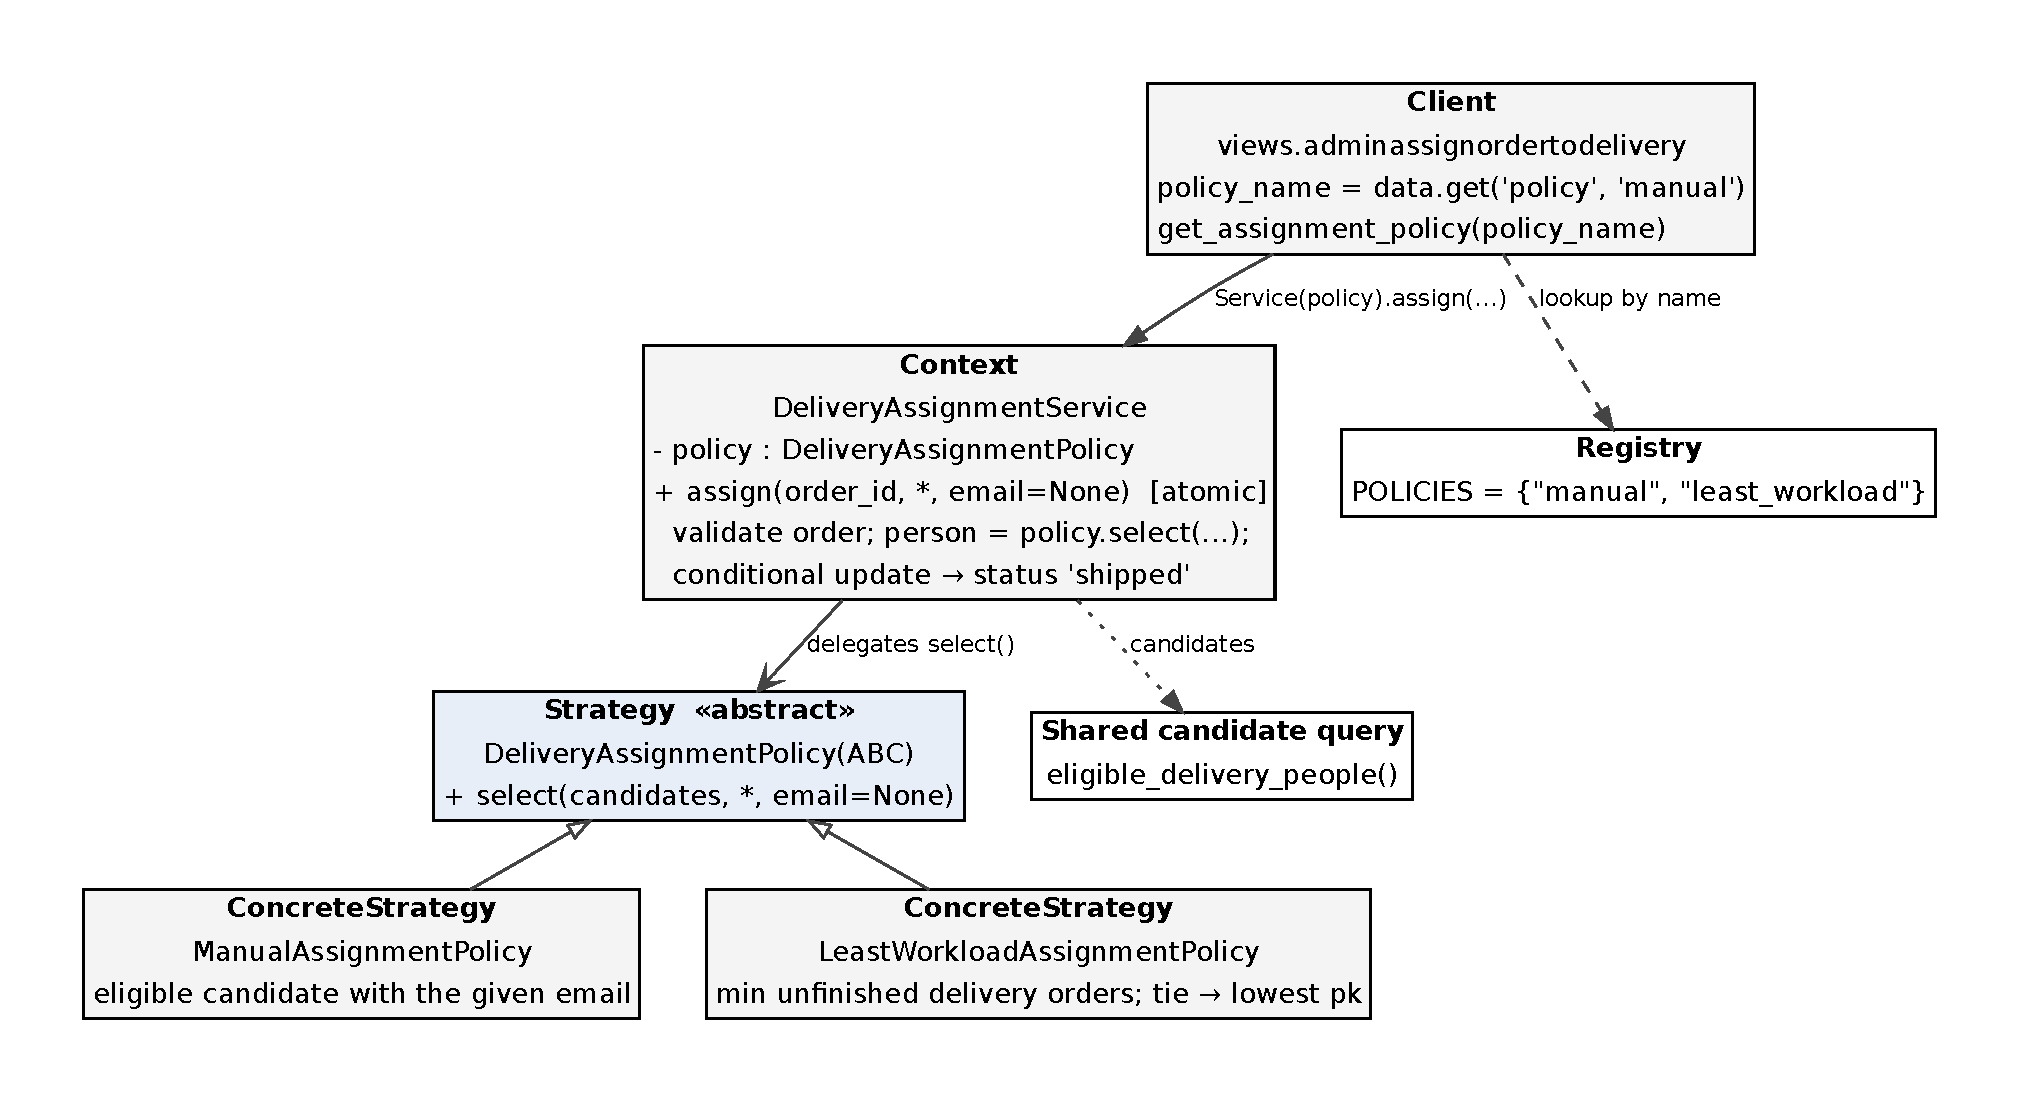
\includegraphics[width=\linewidth]{Part2/diagrams/strategy_delivery_assignment_CH01.pdf}
\caption{Delivery Assignment Policy Selection after CH01. Source: \code{Part2/diagrams/strategy_delivery_assignment_CH01.dot}.}\label{fig:strategy}
\end{figure}

\entry{Refactoring}The baseline view (\code{views.py:1788-1821}) showed several code smells:
\begin{itemize}
\item one function parsed the request, looked up the person and the order, changed the order, printed debug output and published the event;
\item \code{json.loads} had no error handling, so a malformed body caused a server error;
\item a catch-all \code{except Exception} returned HTTP 200 with \code{success: false};
\item nothing stopped a delivered, cancelled or already-assigned order from being reassigned.
\end{itemize}
CH01 applied Extract Class (selection and persistence moved to \code{DeliveryAssignmentService}) and Extract Function (\code{eligible_delivery_people}, \code{_notify_delivery_assignment}) \cite{fowler}, and it replaced the single hard-coded rule with polymorphic policy objects. Three tests show that the existing behaviour survives:
\begin{itemize}
\item \code{test_legacy_manual_payload_and_existing_event} sends the old payload and checks the response, the assigned person, the \code{shipped} status and the original group and event type;
\item \code{test_actual_inmemory_channel_receives_preserved_event} receives that event on the real in-memory layer;
\item \code{test_queue_to_assignment_flow_removes_assigned_order} confirms that the order leaves the assignment queue.
\end{itemize}
Some behaviour changed deliberately: invalid requests now receive 4xx/5xx codes, orders outside the queue are refused, and the write uses \code{QuerySet.update()}. That last choice bypasses \code{Order.save()} and its \code{clean()} call, so a future \code{post_save} receiver for \code{Order} would not see assignments; none exists today.

\entry{Before/after metrics}Both snapshots were measured with the same tool and rules: lizard 1.24.1, counting non-blank, non-comment lines (NLOC) and cyclomatic complexity (CCN) \cite{lizard,mccabe}. Script: \code{Part2/changes/Change1/metrics/measure_ch01.py}; output: \code{ch01_metrics.csv}.

\begin{tabularx}{\linewidth}{@{}Xrr@{}}\toprule
Measure & Baseline & After CH01\\\midrule
\code{views.py} NLOC & 4{,}651 & 4{,}660\\
\code{adminassignordertodelivery} NLOC / CCN & 30 / 5 & 27 / 5\\
\code{delivery_assignment.py} NLOC / maximum function CCN & --- & 77 / 6 (\code{assign})\\
Test code NLOC (\code{test_delivery_assignment.py}) & 0 & 300\\
Diff lines added/removed: module, view, template, tests & \multicolumn{2}{r}{111/0, 41/28, 52/27, 353/0}\\
Application tests passing & no application tests & 39 Django + 9 JS\\\bottomrule
\end{tabularx}

The template is measured by diff lines only, because lizard does not parse Django templates.

\entry{Change and acceptance criteria}\textbf{CH02 and CH03.} The team's files contain no requirement statement or acceptance criteria for these changes. The earlier proposals, \code{data/legacy_datasets/change_scenarios.csv} and \code{Part2/llm/historical_note_evolution_proposals_20260912-064608.md}, list three candidates: notifying new recipients of order-status changes through the Observer collaboration, handling cancellation and refunds as explicit states, and restaurant availability changes.
\entry{Before and after}No commit, diff or changed file exists for either change.
\entry{Implementation and tests}Neither change was implemented, so no test was written or run.
\entry{Pattern effects}None. The counts below have no CH02 or CH03 snapshot.
\entry{Refactoring}None.
\entry{Before/after metrics}Not applicable.

\subsection{Updated pattern counts}\label{sec:counts}
\begin{tabularx}{\linewidth}{@{}Xcccc@{}}\toprule
Snapshot & Types & Instances & Concrete classes & Rejected / uncertain\\\midrule
Baseline (83998629) & 1 & 2 & 3 & 12 / 2\\
After CH01 & 2 & 3 & 5 & 11 / 2\\\bottomrule
\end{tabularx}

After CH01 there are two Observer instances, both preserved under their original names, and one newly introduced Strategy instance. The concrete classes gained are \code{ManualAssignmentPolicy} and \code{LeastWorkloadAssignmentPolicy}, and unique participant symbols rise from 13 to 17. The baseline rejection of manual delivery assignment as a Strategy no longer applies because that code was replaced, which leaves 11 rejected candidates. Records: \code{data/pattern_evolution.csv} and \code{data/pattern_counts.csv}.

\entry{Interpretation}CH01's main benefit is a clear place for new assignment rules: a third policy needs one class and one registry entry, while order checks, the transaction and the notification stay in one place. A test demonstrates this by injecting a policy that the registry does not know. The costs are an extra module to follow, a name-based registry that is checked only at run time, and a context with complexity 6 that now holds state checks the view never had. Production NLOC grew by 86 (77 in the new module and 9 in the view), a figure that says nothing about design quality on its own. ``Least workload'' counts unfinished orders. It does not measure availability, location or shift, because the model has no such fields.

The remaining limits lie outside CH01:
\begin{itemize}
\item \code{pip check} reports six conflicts among the baseline pins, and CH01 was validated in an environment installed with \code{--no-deps};
\item Firebase credentials are absent, and browser rendering was not tested;
\item the assignment event goes to a group that no routed consumer joins;
\item SQLite ignores \code{select_for_update}, so concurrent assignments rely on the conditional write and may return 503.
\end{itemize}
The tests establish that the feature behaves as specified, not that the application is ready to deploy.

\section{Part 3 Cross-language comparison}
\entry{Selected instances}For Observer, \emph{Order Status Broadcast}: the demonstrations' \code{Admin}, \code{Restaurant} and \code{DeliveryPerson} observers correspond to the three consumer groups, and \code{Order.setStatus} plays the role of the notifying view. For Strategy, \emph{Delivery Assignment Policy Selection}, the only confirmed Strategy. The demonstrations predate CH01 and implement the earlier delivery-partner proposal (scenario CS1). Their \code{AvailabilityStrategy} and \code{PriorityStrategy} use \code{available} and \code{priority} attributes that the application's \code{DeliveryPerson} lacks, so they model the pattern structure rather than CH01's two policies. Both programs are simplified models, not translations of the Django code. They are kept unchanged, and their SHA-256 hashes match \code{data/provenance/demonstrations-before.json}.

\entry{Common specifications}The shared fixture is in \code{Part3/test-cases/cases.json}.
\begin{itemize}
\item \textbf{Observer.} Order \code{O101} moves to \code{Shipped} with three observers registered in this order: Admin, Restaurant and \code{DeliveryPerson("Delivery Partner")}. Each observer prints one line, in registration order.
\item \textbf{Strategy.} Partner A is available with priority 2, B is unavailable with priority 5, and C is available with priority 4. The availability rule returns the first available partner (A). The priority rule returns the highest-priority available partner (C), so B is skipped.
\end{itemize}
The expected standard output is in \code{Part3/test-cases/expected_output.txt}. A defined error case is not reachable from the hard-coded fixture: when no partner is available, each language returns its null value and prints ``No delivery partner available''.

\entry{Implementations}Each language has one file under \code{Part3/order_events_and_delivery_selection/} that contains both patterns:
\begin{itemize}
\item \code{java/DesignPatterns.java} (OpenJDK 21.0.12.1);
\item \code{python/design_patterns.py} (CPython 3.13.16);
\item \code{javascript/design-patterns.js} (Node.js 22.22.0);
\item \code{cpp/design_patterns.cpp} (g++ 13.3.0, default flags as in the team's recorded command).
\end{itemize}
Each folder has a \code{README.md} and a \code{run_tests.sh}. The script builds into a temporary directory where needed, runs the program and passes its output to the shared checker \code{Part3/tools/check_output.py}.

\entry{Actual results}All four implementations pass every case: Observer 3/3, Strategy 2/2 and whole-output 1/1, each with exit status 0. Logs: \code{Part3/evidence/test_java.log}, \code{test_python.log}, \code{test_javascript.log} and \code{test_cpp.log}. The earlier table \code{data/legacy_datasets/four_language_execution.csv} records the same outputs without logs.

\entry{Static and dynamic comparison}Markers in \code{Part3/tools/measure.py} split each file into Observer lines, Strategy lines and shared scaffolding (imports, the \code{main} signature, closing braces); the split is saved in \code{Part3/evidence/line_partition.json}. LOC counts non-blank, non-comment lines. CC is lizard's maximum per-function CCN over functions that start in each part (\code{Part3/evidence/static_metrics.csv}, \code{lizard_functions.csv}).

\begin{tabularx}{\linewidth}{@{}lXcccccc@{}}\toprule
 & & \multicolumn{2}{c}{Observer} & \multicolumn{2}{c}{Strategy} & Shared & File\\
Language & Runtime / compiler & LOC & max CC & LOC & max CC & LOC & NLOC\\\midrule
Java & OpenJDK 21.0.12.1 & 45 & 2 & 60 & 5 & 6 & 111\\
Python & CPython 3.13.16 & 31 & 2 & 39 & 4 & 0 & 70\\
JavaScript & Node.js 22.22.0 & 44 & 1 & 49 & 3 & 0 & 93\\
C++ & g++ 13.3.0 & 50 & 2 & 62 & 5 & 7 & 119\\\bottomrule
\end{tabularx}

Timing followed the faculty procedure: compile first, run once to warm up, then take five measured runs on the same machine (Linux 6.18, x86\_64 cloud container) on 2026-10-11. Each figure is the wall-clock time of the whole process. It includes runtime start-up, both pattern sections and output capture, and it excludes compilation. Every measured run produced the expected output (\code{Part3/evidence/timing_raw.csv}).

\begin{tabularx}{\linewidth}{@{}Xrrr@{}}\toprule
Combined Observer + Strategy process & Median (ms) & Min (ms) & Max (ms)\\\midrule
Java (\code{java -cp <build> DesignPatterns}) & 70.7 & 65.2 & 71.9\\
Python (\code{python3 design_patterns.py}) & 18.9 & 15.9 & 20.4\\
JavaScript (\code{node design-patterns.js}) & 34.7 & 32.8 & 40.6\\
C++ (native binary) & 1.9 & 1.8 & 1.9\\\bottomrule
\end{tabularx}

Each program runs both patterns in one process, so the timings are combined figures. For that reason the per-pattern \code{median_process_ms} cells in \code{data/cross_language.csv} are left blank. With so little work per run, the differences reflect the start-up cost of the JVM, Node and CPython rather than the cost of either pattern.

\entry{Comparison}All four programs have the same participants:
\begin{itemize}
\item an Observer type with three concrete observers, and a subject (\code{Order}) that stores a list and iterates over it;
\item a Strategy type with two concrete strategies, and a context that receives its strategy through the constructor.
\end{itemize}
The languages differ first in how strictly the abstraction is declared. Java uses an \code{interface} and C++ an abstract class with pure virtual functions and a virtual destructor, and both compilers enforce them. Python and JavaScript use ordinary base classes with empty methods, so a missing \code{update} surfaces only when it is called. Python's \code{abc} module, which CH01 uses, would make the contract explicit \cite{pyabc}. They also differ in ownership. The C++ subject stores non-owning raw pointers to stack objects, and \code{assign} returns a pointer into the caller's vector that is valid only while that vector exists; the other three languages use garbage-collected references. Complexity is highest in the Java and C++ \code{PriorityStrategy.assign}, at CC~5 (the loop, the \code{if} and two boolean operators). Python's list comprehension with \code{max(key=...)} gives 4, and JavaScript's \code{filter}/\code{reduce} with separate arrow functions gives 3.

\entry{Technology discussion}In the application, Observer is never hand-written; it comes from two framework mechanisms with different guarantees. Django signals run synchronously inside \code{save()}, in the same process and transaction, and are connected when the app loads \cite{djsignals}. Channels groups deliver asynchronously over WebSocket connections and dispatch on the event type. The in-memory layer is intended for development and testing, not for multi-process deployment \cite{channels}. CH01, by contrast, writes Strategy explicitly with \code{abc.ABC}, because no framework hook offers interchangeable selection rules.

\section{LLM records and human verification}
\entry{Run and model}\par
\begin{tabularx}{\linewidth}{@{}lXX@{}}\toprule
Part & Displayed model and date & Record\\\midrule
1a repository selection & not recorded; a link in the note carries \code{utm_source=chatgpt.com} & pasted output only\\
1b pattern analysis & not recorded; same indication & pasted output only\\
2 change proposals & not recorded; the file name holds the paste time 2026-09-12 06:46 & pasted output only\\
Report production & Claude Opus 5.5 in the Claude app (identifier \code{claude-opus-5-5}), 2026-10-11; Claude Pro plan & two exact prompts saved\\\bottomrule
\end{tabularx}

Canonical records: \code{data/llm.csv}. For the three historical analyses only pasted outputs survive, and they are recorded as such.

\entry{Inputs and outputs}Historical outputs are in \code{Part1/llm/historical_note_repository_selection.md}, \code{Part1/llm/historical_note_pattern_analysis.md} and \code{Part2/llm/historical_note_evolution_proposals_20260912-064608.md}; the inputs given to those sessions were not recorded. For report production, the exact prompts are \code{data/llm/2026-10-11_report_generation_prompt.md} and \code{data/llm/2026-10-11_report_revision_prompt.md}. The supplied files, with their hashes and the source commit 83998629, are listed in \code{data/llm/2026-10-11_report_generation_inputs.md}. The outputs are this report, the CSV datasets, the README, the diagrams and the measurement scripts.

\entry{Claims and evaluation}
\begin{itemize}
\item \textbf{Part~1b note: partially correct.} It rightly identifies the Channels broadcast as Observer-like and rejects State, Strategy, Facade, Singleton, Adapter, Factory, Command, Repository and Template Method. It misses the \code{post_save} collaboration, does not separate the publish--subscribe form from strict Observer, and overlooks that the subscriber of the assignment event is disabled inside a string literal (\code{Part1/evidence/candidate_scan.txt}).
\item \textbf{Part~2 note: partially correct, as a set of proposals.} Its Strategy proposal was implemented in CH01 with different policies, because the model has no availability or priority fields. Its other proposals remain unimplemented.
\item \textbf{Part~1a note: cannot fully confirm.} Its description of the chosen repository matches the code, but its claims about the other repositories were not re-checked.
\item \textbf{Report production: requires team review.} Each figure in this report was traced to a log or a script output.
\end{itemize}

\entry{Generated code}The team states that no AI tool was used to write the CH01 code or the four demonstrations. The report-production session wrote the Part~3 test runners and checker, \code{Part3/tools/measure.py}, \code{Part1/evidence/scan_candidates.sh}, \code{Part2/changes/Change1/metrics/measure_ch01.py}, \code{data/code/verify_baseline.py} and the Graphviz diagram sources. Each was executed, and its output is stored beside it. None of them modifies the application or the demonstrations.

\section{Findings, contributions and references}
\entry{Findings}
\begin{enumerate}
\item At commit 83998629 the application contains one confirmed pattern, Observer, in two instances. Both rely on framework mechanisms rather than hand-written subjects: Django's \code{post_save} signal for cart cleanup and Channels groups for live order updates.
\item The subject role in the order broadcast is spread over five view functions that publish to the same groups. New observers are easy to add, but the sending side is repetitive: \code{adminupdateorderstatus} sends eight events for every status change.
\item The delivery-assignment notification has no live subscriber at the baseline, because its only consumer is disabled inside a string literal and is not routed. CH01 preserves the event as it was.
\item CH01 introduces a Strategy with a clear abstraction, two policies and a context that owns validation and persistence. 39 Django tests and 9 script tests pass in the recorded validation environment.
\item The four-language demonstrations produce identical results on the shared fixture. Their timings mainly reflect runtime start-up.
\end{enumerate}
\entry{Contributions}\par
{\small\begin{tabularx}{\linewidth}{@{}lp{0.15\linewidth}lp{0.2\linewidth}X@{}}\toprule
Roll number & Name & Batch & Contribution & Source and evidence\\\midrule
AM.SC.U4CSE23001 & Aadil Nizar & CSE A & Refactoring and CH01 implementation & \code{Part2/changes/Change1/}, \code{data/code/evolved_CH01/}\\
AM.SC.U4CSE23007 & Adil Najeem & CSE A & Baseline analysis & \code{data/code/baseline_83998629/}, \code{data/provenance/}, Section~1\\
AM.SC.U4CSE23014 & Athul Yesudas & CSE A & Pattern discovery & \code{Part1/}, \code{data/patterns.csv}\\
AM.SC.U4CSE23039 & Hima C & CSE A & Testing and validation & \code{Part2/changes/Change1/evidence/}, \code{Part3/evidence/}\\
AM.SC.U4CSE23046 & M Krishnapriya & CSE A & Cross-language comparison & \code{Part3/}, \code{data/cross_language.csv}\\
AM.SC.U4CSE23053 & Muhammed Faais A & CSE A & Report and repository preparation & \code{A1_Report.tex}, \code{README.md}, \code{data/}\\\bottomrule
\end{tabularx}}

\entry{References}
\renewcommand{\refname}{}\vspace{-2.5em}
\begin{thebibliography}{9}\small
\bibitem{app} H.~Vemali, \emph{campus-food-ordering} (Canteen Management System), GitHub, commit 83998629e633594037cfa25e583542f9f6f0f968, MIT licence. \url{https://github.com/HarshavardhanVemali/campus-food-ordering}
\bibitem{gof} E.~Gamma, R.~Helm, R.~Johnson and J.~Vlissides, \emph{Design Patterns: Elements of Reusable Object-Oriented Software}. Addison-Wesley, 1994 (Observer, pp.~293--303; Strategy, pp.~315--323).
\bibitem{djsignals} Django Software Foundation, ``Signals'', Django 6.0 documentation. \url{https://docs.djangoproject.com/en/6.0/topics/signals/} (accessed 2026-10-11).
\bibitem{channels} Django Channels, ``Channel Layers'', Channels documentation. \url{https://channels.readthedocs.io/en/latest/topics/channel_layers.html} (accessed 2026-10-11).
\bibitem{eip} G.~Hohpe and B.~Woolf, \emph{Enterprise Integration Patterns}. Addison-Wesley, 2003 (Publish-Subscribe Channel).
\bibitem{fowler} M.~Fowler, \emph{Refactoring: Improving the Design of Existing Code}, 2nd ed. Addison-Wesley, 2018 (Extract Class, Extract Function).
\bibitem{mccabe} T.~J.~McCabe, ``A complexity measure'', \emph{IEEE Transactions on Software Engineering}, SE-2(4):308--320, 1976.
\bibitem{lizard} T.~Yin, \emph{lizard} code complexity analyser, version 1.24.1. \url{https://github.com/terryyin/lizard}
\bibitem{pyabc} Python Software Foundation, ``abc --- Abstract Base Classes'', Python 3 documentation. \url{https://docs.python.org/3/library/abc.html}
\end{thebibliography}

\section{Team folder and datasets (take a screenshots from the GitHub repository— your team)}
Figure~\ref{fig:repo} shows the team folder on GitHub after the first upload (commit \code{82a5d58}, ``A1 SUBMISSION''). The folder contains the report, its LaTeX source, the README and the four folders below; the screenshot image is stored at \code{data/test_result/github_team_folder_82a5d58.png}.

\begin{figure}[H]\centering
\makebox[\linewidth]{\setlength{\fboxsep}{0pt}\setlength{\fboxrule}{0.4pt}\fbox{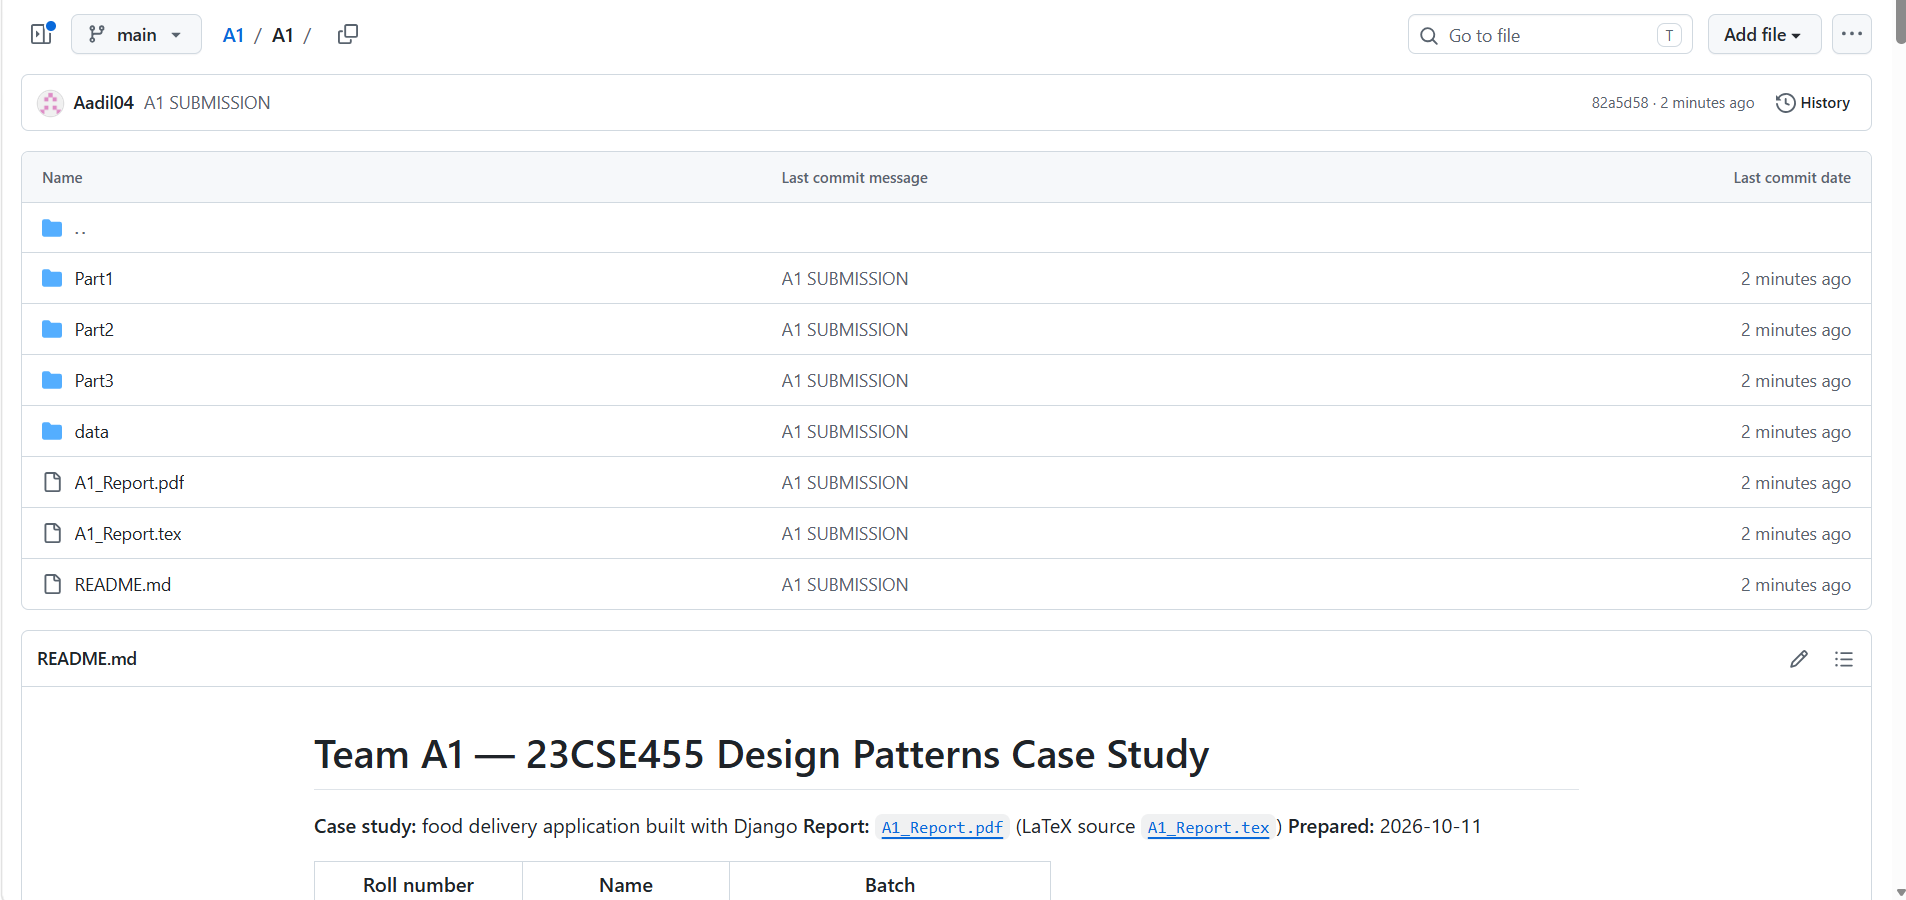
\includegraphics[width=180mm,keepaspectratio]{data/test_result/github_team_folder_82a5d58.png}}}
\caption{GitHub listing of the team folder (breadcrumb ``A1 / A1'', branch \code{main}) after commit \code{82a5d58}, ``A1 SUBMISSION'' by Aadil04. It shows \code{Part1/}, \code{Part2/}, \code{Part3/}, \code{data/}, \code{A1_Report.pdf}, \code{A1_Report.tex} and \code{README.md}, with the start of the rendered README below.}\label{fig:repo}
\end{figure}
\begin{verbatim}
A1/
  README.md, A1_Report.tex, A1_Report.pdf
  data/   patterns.csv, pattern_counts.csv, pattern_evolution.csv,
          cross_language.csv, llm.csv
          code/baseline_83998629/   original application
          code/evolved_CH01/        application after CH01
          provenance/, legacy_datasets/, llm/, test_result/
  Part1/  pattern_architecture/, evidence/, llm/
  Part2/  changes/Change1/ (requirement, diff, source, tests, logs, metrics),
          changes/Change2/, changes/Change3/, diagrams/, llm/
  Part3/  order_events_and_delivery_selection/{java,python,javascript,cpp}/,
          test-cases/, tools/, evidence/, llm/
\end{verbatim}
The faculty documents give some datasets more than one name (\code{Pattern_count.csv}, \code{patterns_evolution.csv}, \code{pattern_evalution.csv}, \code{pattern_crosslanguage.csv}) and ask that the CSVs not be repeated inside the part folders. One canonical copy of each is therefore kept in \code{data/}, with the column names exactly as given in the instructions; the name mapping is recorded in \code{README.md}.


\end{document}
